\section{Die Bibel}
\subsection{Grundlegendes}
\subsubsection{Was ist die Bibel?}
Die Bibel ist das meist verkaufte Buch auf dieser Welt. Ob es auch das meist gelesene ist? Wasser aber sicher ist, es das meist untersuchte Buch. Jeder einzeln Buchstabe, jedes Wort und jeder Satz wurde auf das genaueste Untersucht.

In früheren Zeiten wo das Buch noch abgeschrieben werden musste, weil der Buchdruck noch nicht erfunden wurde, wurde jeder einzelne Buchstabe gezählt. Wenn bei der Kontrolle die Anzahl nicht stimmte, war man sicher das diese Ausgabe nicht stimmen kann. Bis ins kleinste Detail wurde aufgepasst, dass die Abschrift genau dem Original übereinstimmt.
\begin{figure}
    \centering
    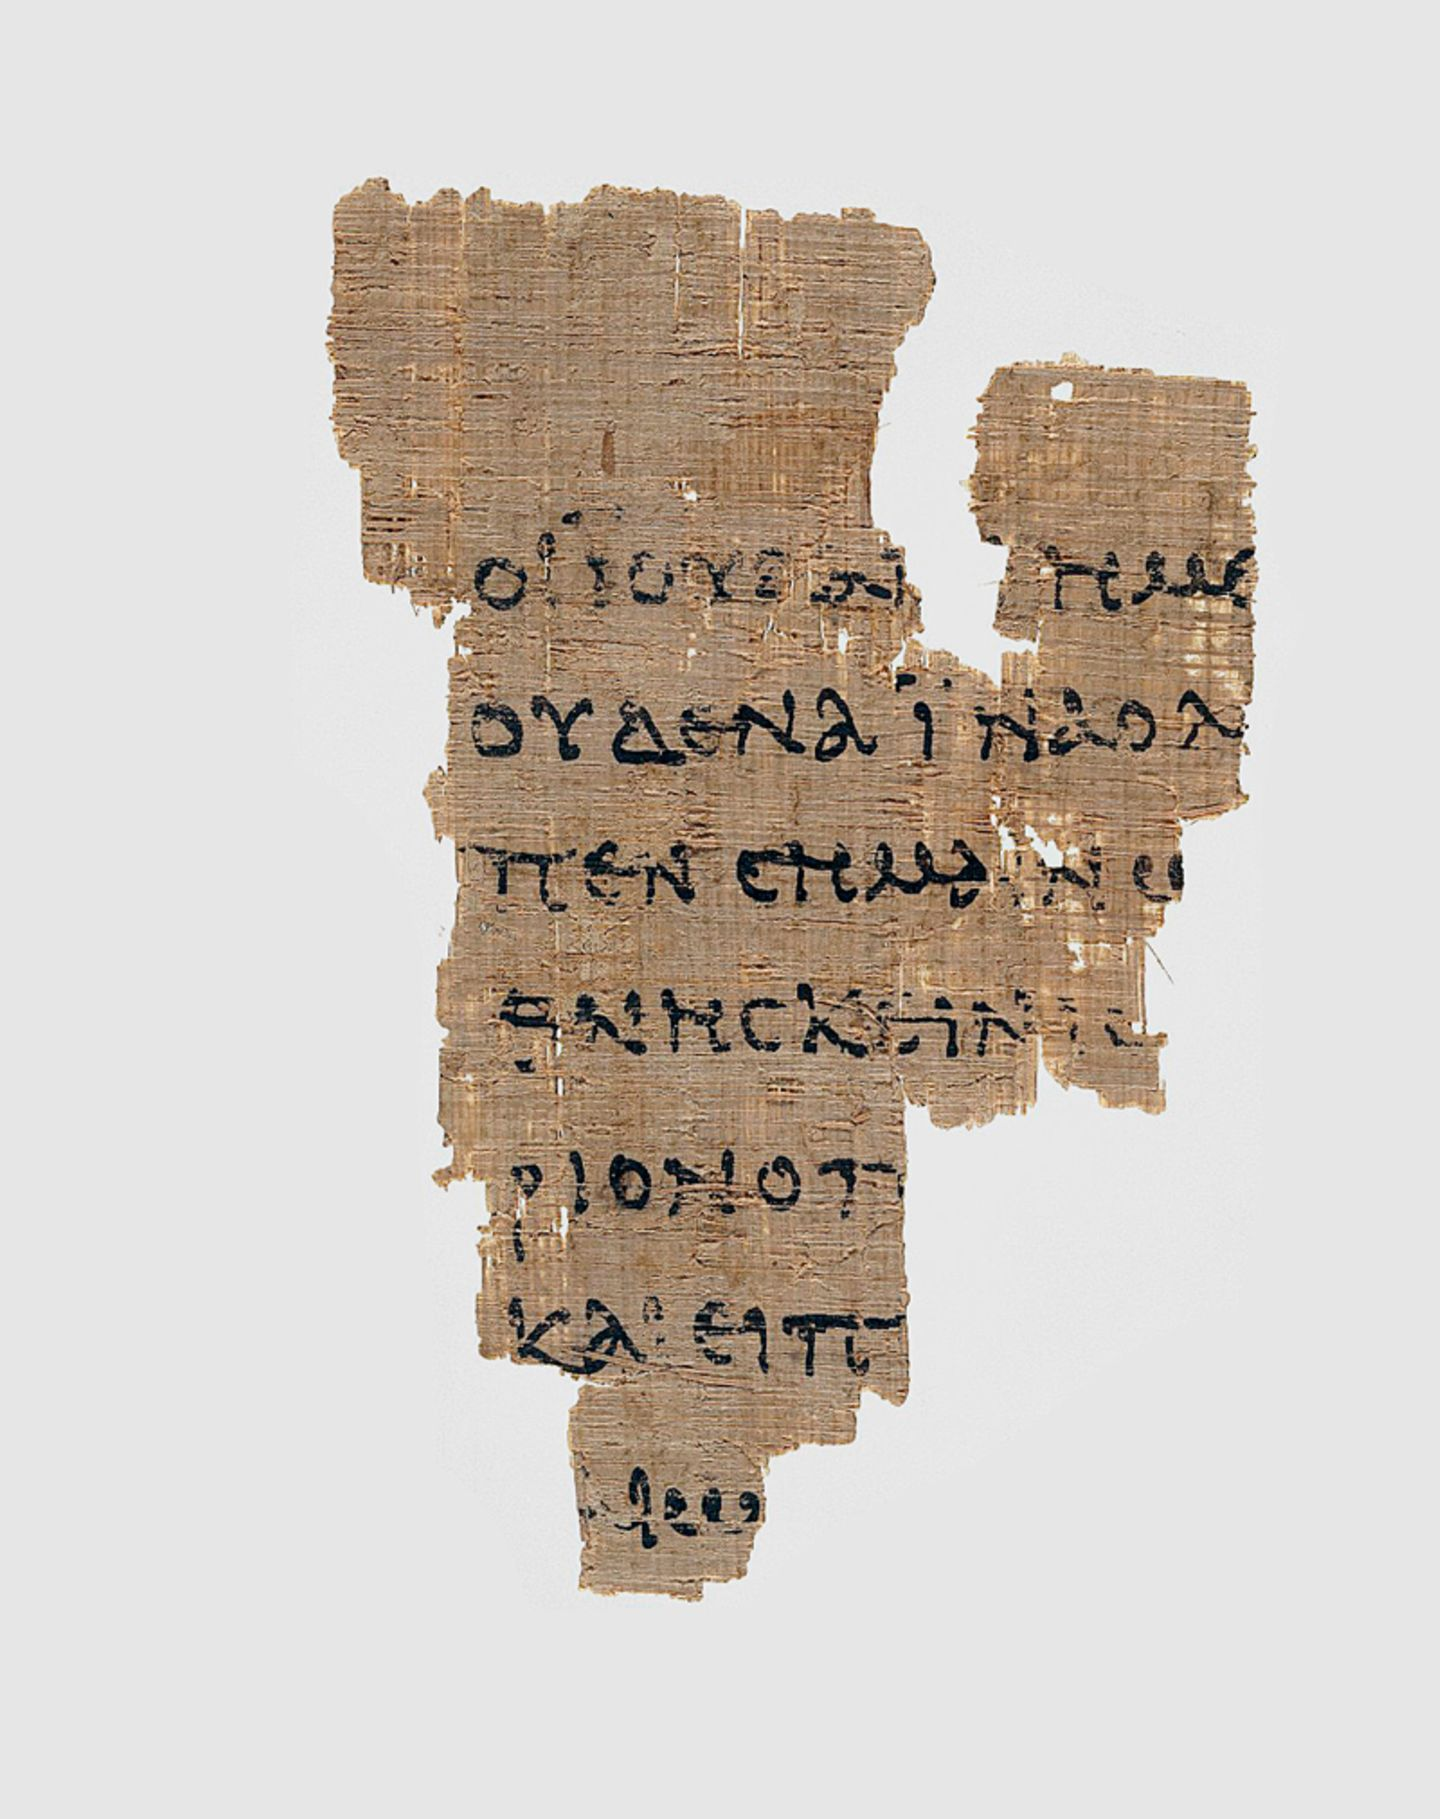
\includegraphics[width=0.5\linewidth]{src/Vorträge/BibelBuch/images/papyrusFragment.jpg}
    \caption{Dieses Papyrusfragment von etwa 125 n. Chr. ist der älteste Beleg für das Neue Testament. Er handelt vom Prozess gegen Jesus: Die Frage »Bist du der König der Juden?« ist teilweise zu entziffern\\
©John Rylands Library}
    \label{fig:enter-label}
\end{figure}